\documentclass[11pt]{article}
\usepackage{placeins}
\usepackage{graphicx}
\usepackage{url}

\begin{document}

\begin{titlepage}
	\begin{center}
    	
\includegraphics[scale=0.10]{du.png}\par
		\begin{Huge}
			\textsc{University of Dhaka}\par
		\end{Huge}
		\begin{Large}
			Department of Computer Science and Engineering\par \vspace{1cm}
			CSE-3111 : Computer Networking Lab \\[12pt]	
			Lab Report X : Introduction to Socket Programming — Exercises on Simple Client-Server Communication
		\end{Large}
	\end{center}  	
	\begin{large}
		\textbf{Submitted By:\\[12pt]}
			Name : Tasfia Tabassum\\[8pt]
			Roll No : 24\\[12pt]
			Name : Saima Akter\\[8pt]
			Roll No : 30\\[12pt]
		\textbf{Submitted On : \\[12pt]}
			January 24, 2023\\[20pt]
		\textbf{Submitted To :\\[12pt]}
			Dr. Md. Abdur Razzaque\\[12pt]
                Md Mahmudur Rahman\\[12pt]
                Md. Ashraful Islam\\[12pt]
                Md. Fahim Arefin
	\end{large}
\end{titlepage}

\section{Introduction}
In Client and Server setup where a Client connects, sends messages to the server and the server shows them using a socket connection. There’s a lot of low-level stuff that needs to happen for these things to work but the Java API networking package (java.net) takes care of all of that, making network programming very easy for programmers.

\subsection{Objectives}
Write down two or three specific objectives of this lab experiment.
\begin{itemize}
    \item Get idea regarding socket programming.
    \item Learn about client-server communication.
\end{itemize}
%%%%
%%%%

\section{Establishing a socket connection between a server and a client}
\subsection{Java program for a Server }
To write a server application two sockets are needed. 

    A ServerSocket which waits for the client requests (when a client makes a new Socket())
    A plain old Socket to use for communication with the client: \\[12pt]

Communication\\[6pt] 
getOutputStream() method is used to send the output through the socket. the data. \\[2pt]

Closing the connection\\[6pt]

After finishing,  it is important to close the connection by closing the socket as well as input/output streams.\\[12pt]

\pagebreak

\textbf{Java Implementation}\\[12pt]

\begin{verbatim}
import java.net.*;
import java.io.*;

public class Server {
    private DataInputStream input = null;
    private DataOutputStream out = null;
    private Socket socket = null;
    private ServerSocket server = null;
    private DataInputStream in = null;

    public Server(int port) {
        try {
            server = new ServerSocket(port);
            System.out.println("Server started");

            System.out.println("Waiting for a client ...");

            socket = server.accept();
            System.out.println("Client accepted");
            in = new DataInputStream(
                    new BufferedInputStream(socket.getInputStream()));

            String line = "";
            while (!line.equals("Over")) {
                try {
                    in = new DataInputStream(System.in);
                    out = new DataOutputStream(
                            socket.getOutputStream());

                    line = in.readUTF().toUpperCase();
                    System.out.println(line);
                    line = in.readLine();
                    out.writeUTF(line);


                } catch (IOException i) {
                    System.out.println(i);
                }
            }
            System.out.println("Closing connection");

            // close connection
            socket.close();
            in.close();
        } catch (IOException i) {
            System.out.println(i);
        }
    }

    public static void main(String args[]) {
        Server server = new Server(5000);
    }
}
\end{verbatim}

 Output : 
  \begin{figure}[!h]
\centering
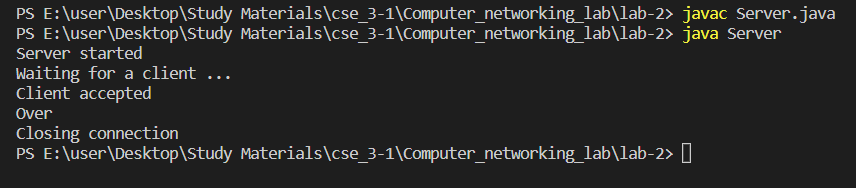
\includegraphics[width=\textwidth]{server.png}
\caption{Java program for a Server}
\end{figure}
\FloatBarrier


\subsection{Java program for a Client}
To connect to another machine we need a socket connection. A socket connection means the two machines have information about each other’s network location (IP Address) and TCP port. The java.net.Socket class represents a Socket. To open a socket: \\[12pt]

Socket socket = new Socket(“127.0.0.1”, 5000)\\[12pt]

    The first argument – IP address of Server. ( 127.0.0.1  is the IP address of localhost, where code will run on the single stand-alone machine).\\[6pt]
    The second argument – TCP Port. (Just a number representing which application to run on a server. For example, HTTP runs on port 80. Port number can be from 0 to 65535)\\[12pt]

Communication\\[6pt] 
To communicate over a socket connection, streams are used to both input and output the data. \\[2pt]

Closing the connection\\[6pt]

The socket connection is closed explicitly once the message to the server is sent.\\[12pt]

\textbf{Java Implementation}\\[12pt]

\begin{verbatim}
import java.io.*;
import java.net.*;

public class Client {
	private Socket socket = null;
	private DataInputStream input = null;
	private DataOutputStream out = null;
	public Client(String address, int port)
	{
		try {
			socket = new Socket(address, port);
			System.out.println("Connected");
			input = new DataInputStream(System.in);

			// sends output to the socket
			out = new DataOutputStream(
				socket.getOutputStream());

                String line = "" ;

            line = input.readUTF();
                    System.out.println(line);


		}
		catch (UnknownHostException u) {
			System.out.println(u);
			return;
		}
		catch (IOException i) {
			System.out.println(i);
			return;
		}
		String line = "";
		while (!line.equals("Over")) {
			try {
				line = input.readLine();
				out.writeUTF(line);
			}
			catch (IOException i) {
				System.out.println(i);
			}
		}

		// close the connection
		try {
			input.close();
			out.close();
			socket.close();
		}
		catch (IOException i) {
			System.out.println(i);
		}
	}

	public static void main(String args[])
	{
		Client client = new Client("192.168.1.103", 5000);
	}
}
\end{verbatim}

 Output : 
\begin{figure}[!h]
\centering
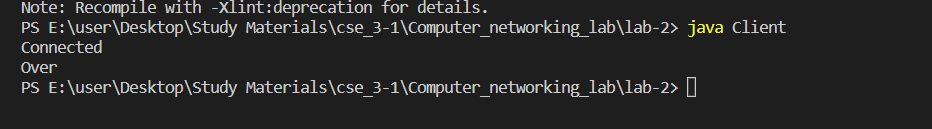
\includegraphics[width=\textwidth]{client.png}
\caption{Java program for a Client}
\end{figure}
\FloatBarrier


\section{Small letter to capital letter conversion}
\subsection{Java program for a Server}
Java Implementation \\[2pt]
\begin{verbatim}
    
import java.io.*;
import java.net.*;

public class upper_case_server{

    public static void main (String[] args) throws IOException {

        System.out.println("Server started");
        System.out.println("Waiting for Clients...");
        ServerSocket serverSocket = new ServerSocket (5000);
        Socket clientSocket = serverSocket.accept ();

        BufferedReader in = new BufferedReader (new InputStreamReader 
        (clientSocket.getInputStream ()));
        PrintWriter out = new PrintWriter(clientSocket.getOutputStream(), true);
        String message, modifiedMessage;
        message = in.readLine ();
        System.out.print("The received message from client: " + message);
        modifiedMessage = message.toUpperCase();
        out.println(modifiedMessage);
        System.out.println ("\nModified message which is sent to client: " + 
        modifiedMessage);
    }

}
\end{verbatim}

 Output : 
\begin{figure}[!h]
\centering
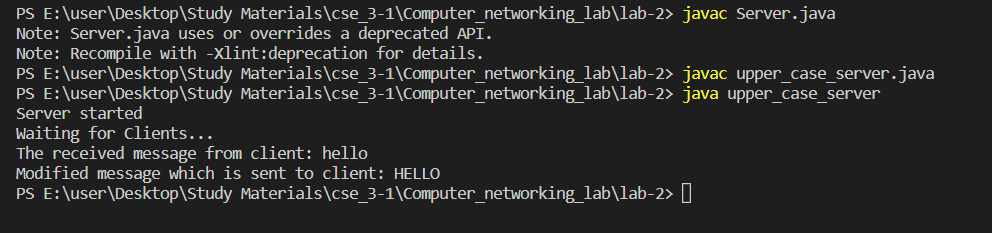
\includegraphics[width=\textwidth]{upper_server.png}
\caption{Java program for a Server}
\end{figure}
\FloatBarrier

\subsection{Java program for a Client}
Java Implementation \\[2pt]
\begin{verbatim}
import java.io.*;
import java.net.*;

public class upper_case_client {

    public static void main(String[] args) throws IOException {
        System.out.println("Started");
        Socket socket = new Socket("192.168.1.103", 5000);
        System.out.println("Client Connected with Server");
        PrintWriter out = new PrintWriter(socket.getOutputStream(), true);
        System.out.println("Enter a lowercase sentence: ");
        BufferedReader reader = new BufferedReader(new InputStreamReader(System.in));
       BufferedReader in = new BufferedReader((new 
       InputStreamReader(socket.getInputStream())));

        String messageSent = reader.readLine();
        System.out.println("The message sent is: " + messageSent);
        out.println(messageSent);


        String messageReceived = in.readLine();
        System.out.println("The modified message is: " + messageReceived);
    }
}
\end{verbatim}


 Output : 
\begin{figure}[!h]
\centering
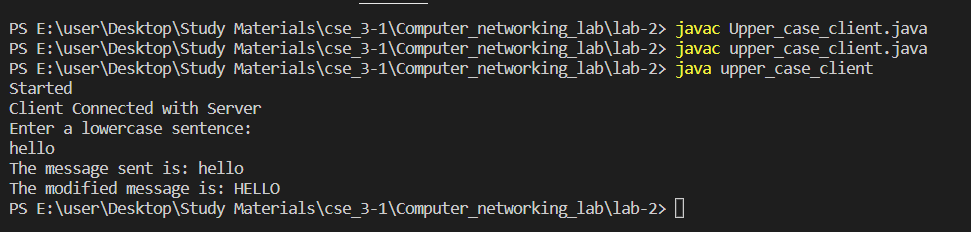
\includegraphics[width=\textwidth]{upper_client.png}
\caption{Uppercase Client}
\end{figure}
\FloatBarrier

\section{Checking whether a number is prime or not}
\subsection{Java program for a Server }
Java Implementation \\[2pt]
\begin{verbatim}

import java.net.*;
import java.io.*;

public class prime_server
{
    public static void main(String args[]) throws IOException
    {
        System.out.println("Server started");
        System.out.println("Waiting for Clients...");
        ServerSocket serverSocket = new ServerSocket(5000);

        Socket socket = serverSocket.accept();
        System.out.println("Client Accepted");
        ObjectInputStream ois = new ObjectInputStream(socket.getInputStream());
        ObjectOutputStream oos = new ObjectOutputStream(socket.getOutputStream());

        try{
            Object cMsg = ois.readObject();
            System.out.println("From Client: " + (int)cMsg);

            int serverMsg = (int) cMsg;
//            serverMsg = serverMsg.toUpperCase();

            boolean ans = isPrime(serverMsg);

            if (ans==true)
                oos.writeObject("The number is prime");
            else
                oos.writeObject("The number is not prime");
        }
        catch(Exception e)
        {
            e.printStackTrace();
        }
    }
    static boolean isPrime(int num)
    {
        if(num<=1)
        {
            return false;
        }
        for(int i=2;i<=num/2;i++)
        {
            if((num%i)==0)
                return  false;
        }
        return true;
    }
}
\end{verbatim}
\pagebreak
 Output : 
\begin{figure}[!h]
\centering
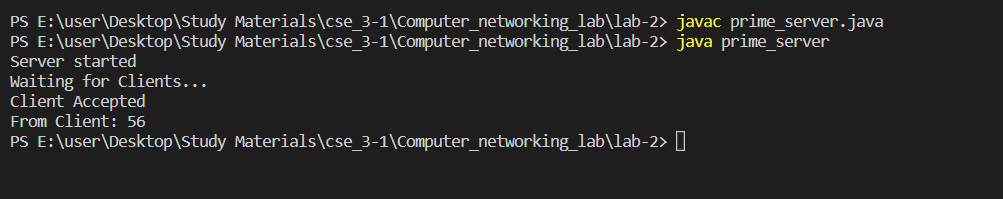
\includegraphics[width=\textwidth]{prime_server.png}
\caption{Prime Server}
\end{figure}
\FloatBarrier


\subsection{Java program for a Client }
Java Implementation \\[2pt]
\begin{verbatim}
import java.io.IOException;
import java.io.ObjectInputStream;
import java.io.ObjectOutputStream;
import java.net.Socket;
import java.util.Scanner;

public class prime_client {
    public static void main(String[] args) throws IOException, 
    ClassNotFoundException {
        System.out.println("Started");
        Socket socket = new Socket("192.168.1.103", 5000);
        System.out.println("Client Connected with Server");

        ObjectOutputStream objectOutputStream = new 
        ObjectOutputStream(socket.getOutputStream());
        ObjectInputStream objectInputStream = new 
        ObjectInputStream(socket.getInputStream());

        Scanner scanner = new Scanner(System.in);
        System.out.println("Enter a number to check prime or not:");
        int number = scanner.nextInt();

        objectOutputStream.writeObject(number);

        try {
            Object fromServer = objectInputStream.readObject();
            System.out.println("From server : " + (String) fromServer);
        } catch (IOException e) {
            throw new RuntimeException(e);
        } catch (ClassNotFoundException e) {
            throw new RuntimeException(e);
        }
    }
}
\end{verbatim}




 Output : 
\begin{figure}[!h]
\centering
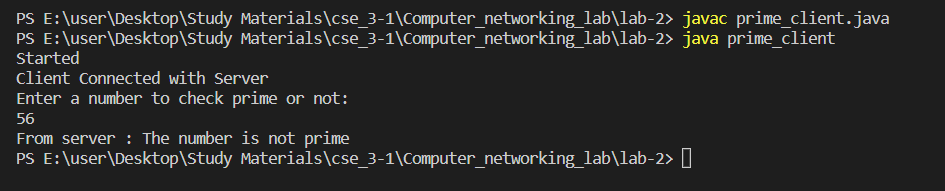
\includegraphics[width=\textwidth]{prime_client.png}
\caption{Prime Client}
\end{figure}
\FloatBarrier


\section{ATM Client-Server Communication}
This is an application-level protocol to be used between an
automatic teller machine and a bank’s centralized server. Our protocol are
allow a user’s card and password to be verified, the account balance (which is
maintained at the centralized computer) to be queried, and an account
withdrawal to be made (that is, money disbursed to the user). Our protocol
entities are able to handle the all-too-common cases in which there is not
enough money in the account to cover the withdrawal. Our protocol by
listing the messages exchanged and the action taken by the automatic teller
machine or the bank’s centralized computer on transmission and receipt of
messages.\\[12pt]
it can handle errors related
to both request and response messages to and from the server.

\subsection{Java program for a Server }
Java Implementation \\[2pt]

\begin{verbatim}
import java.net.*;
import java.io.*;
import java.util.concurrent.TimeUnit;

public class atm_server {
    String username;
    String password;
    int balance;
    int req_id;

    atm_server(String username, String password, int balance) {
        this.username = username;
        this.password = password;
        this.balance = balance;
    }

    public void setBalance(int newBalance) {
        this.balance = newBalance;
    }

    public int getBalance() {
        return this.balance;
    }

    public int getReq_id() {
        return this.req_id;
    }

    public void setReq_id() {
        this.req_id = getReq_id() + 1;
    }

    public String checkBalance() {
        return "Your current balance is: " + getBalance() + " taka";
    }

    public void credit(int value) {
        setBalance(getBalance() + value);
    }

    public boolean debit(int value) {
        if (getBalance() >= value) {
            setBalance(getBalance() - value);
            return true;
        } else
            return false;
    }

    public static void main(String args[]) throws IOException {
        int userNo = -1;

        atm_server[] users;

        users = new atm_server[3];

        users[1] = new atm_server("saima", "tonni", 3000);
        users[0] = new atm_server("tasfia", "tabassum", 6000);

        delay();

        System.out.println("Server started");

        delay();

        System.out.println("Waiting for Clients to connect");

        ServerSocket serverSocket = new ServerSocket(5000);
        Socket socket = serverSocket.accept();
        delay();
        System.out.println("Client Accepted");
        ObjectInputStream ois = new ObjectInputStream(socket.getInputStream());
        ObjectOutputStream oos = new ObjectOutputStream(socket.getOutputStream());

        try {
            Object message1 = ois.readObject();
            Object msg2 = ois.readObject();

            String Name = (String) message1;
            String Password = (String) msg2;

            for (int i = 0; i < 3; i++) {
                if (Name.equals(users[i].username) && 
                Password.equals(users[i].password)) {
                    oos.writeObject(true);
                    userNo = i;
                    break;
                } else
                    oos.writeObject(false);
            }
            while (true) {
                Object cMsg3 = ois.readObject();
                String command = (String) cMsg3;

                if (userNo >= 0) {
                    if (command.equals("Credit")) {

                        sendPackets();

                        oos.writeObject("Enter amount to be credited:\n");

                        Object cMsg4 = ois.readObject();
                        int value = (int) cMsg4;

                        users[userNo].credit(value);

                        sendPackets();

                        oos.writeObject("Your account has been credited by " + value + " tk\n"
                                + users[userNo].checkBalance());

                    } else if (command.equals("Debit")) {

                        sendPackets();

                        oos.writeObject("Enter amount to be debited:\n");

                        Object cMsg4 = ois.readObject();
                        int value = (int) cMsg4;

                        sendPackets();

                        if (users[userNo].debit(value) == true)
                            oos.writeObject("Your account has been debited by " +
                            
                            value + " tk\n"
                                    + users[userNo].checkBalance());
                        else
                            oos.writeObject("Balance is not sufficient\n" + 
                            users[userNo].checkBalance());
                    } else if (command.equals("Quit")) {

                        sendPackets();

                        oos.writeObject("Log Out Successful...\n");

                        delay();

                        System.out.println("System shutting down...\n");

                        break;
                    } else if (command.equals("Balance")) {

                        sendPackets();

                        oos.writeObject(users[userNo].checkBalance());
                    }
                }
            }
        } catch (Exception e) {
            e.printStackTrace();
        }
    }

    static boolean error() {

        int num = (int) Math.floor(Math.random() * (100));

        if (num < 50) {
            delay();
            System.out.println("\nData sent successfully to the Client...\n");
            return true;
        } else {
            delay();
            System.out.println("\nData not sent to the Client\nTrying again to 
            sent...\n");
            return false;
        }
    }

    static void sendPackets() {
        while (true) {
            if (error() == true)
                break;
        }
    }

    static void delay() {
        try {
            Thread.sleep(1000);
        } catch (InterruptedException e) {
            e.printStackTrace();
        }
    }
}
\end{verbatim}

 Output : 
\begin{figure}[!h]
\centering
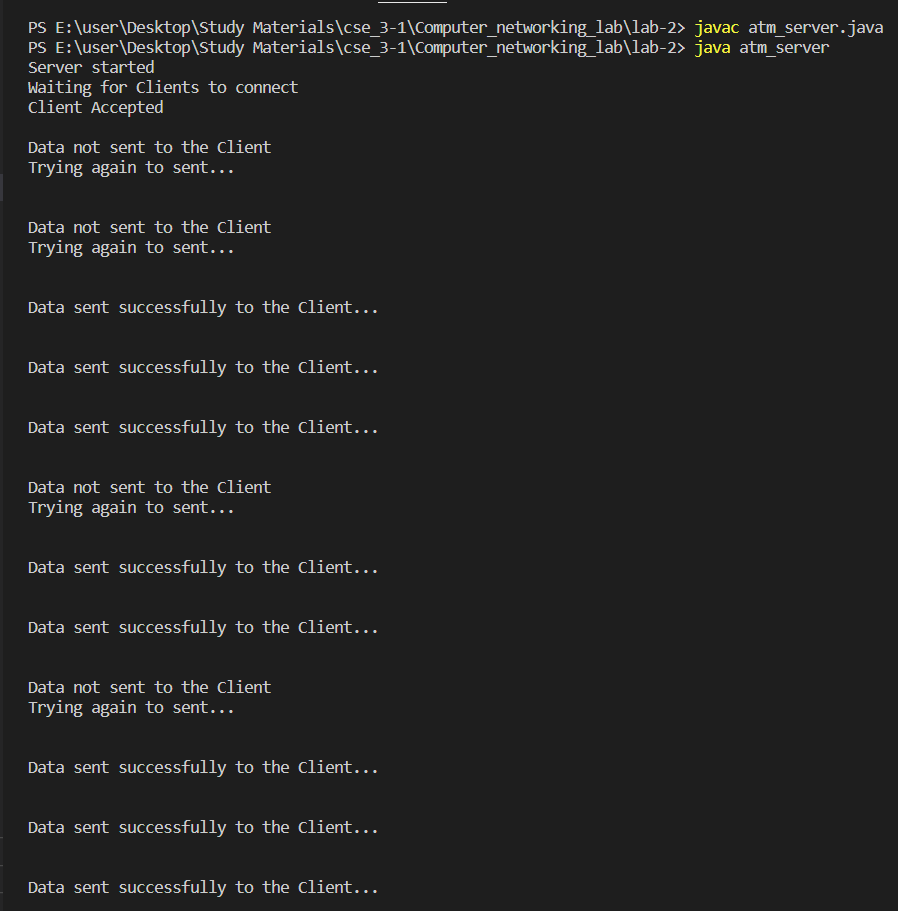
\includegraphics[width=\textwidth]{atm_server.png}
\caption{ATM Server}
\end{figure}
\FloatBarrier

\subsection{Java program for a Client}
Java Implementation \\[2pt]
\begin{verbatim}
import java.io.IOException;
import java.io.ObjectInputStream;
import java.io.ObjectOutputStream;
import java.lang.Math;
import java.net.Socket;
import java.util.Scanner;
import java.util.concurrent.TimeUnit;

public class atm_client {
    public static void main(String[] args) throws IOException, 
    ClassNotFoundException {
        delay();
        System.out.println("Client");
        Socket socket = new Socket("192.168.117.150", 5000);

        Scanner scanner = new Scanner(System.in);
        delay();
        System.out.println("Client Connected successfully");
        delay();
        System.out.println("Enter username:");
        String name = scanner.nextLine();
        delay();
        System.out.println("Enter password:");
        String pass = scanner.nextLine();

        ObjectOutputStream objectOutputStream = new 
        ObjectOutputStream(socket.getOutputStream());
        ObjectInputStream objectInputStream = new 
        ObjectInputStream(socket.getInputStream());

        objectOutputStream.writeObject(name);
        objectOutputStream.writeObject(pass);

        Object fromServer1 = objectInputStream.readObject();

        if ((boolean) fromServer1 == true) {
            delay();
            System.out.println("\nLogin Successful...");

            String str;
            int val;

            while (true) {

                delay();

                System.out.println("\nChoose Option please:\n");
                System.out.println("Press 'Balnace' to check balance");
                System.out.println("Press 'Credit' to Credit balance");
                System.out.println("Press 'Debit' to Debit balance");
                System.out.println("Press 'Quit' to Log Out\n");

                str = scanner.nextLine();
                objectOutputStream.writeObject(str);

                sendPackets();

                if (str.equals("Quit")) {
                    delay();
                    Object fromServer = objectInputStream.readObject();
                    System.out.println("\n" + fromServer);

                    break;
                }
                try {
                    delay();
                    Object fromServer = objectInputStream.readObject();
                    System.out.println("\n" + fromServer);

                    if (str.equals("Credit") || str.equals("Debit")) {

                        val = scanner.nextInt();
                        scanner.nextLine();
                        objectOutputStream.writeObject(val);

                        sendPackets();

                        try {
                            Object fromServer2 = objectInputStream.readObject();
                            delay();
                            System.out.println("\n" + fromServer2);
                        } catch (Exception e) {
                            e.printStackTrace();
                        }
                    }

                } catch (Exception e) {
                    e.printStackTrace();
                }
            }
        }

        else {
            delay();
            System.out.println("Login Failed! Try again...");
            System.exit(0);
        }
    }

    static boolean error() {

        int num = (int) Math.floor(Math.random() * (100));

        if (num < 50) {
            delay();
            System.out.println("\nData sent successfully to the Server...\n");
            return true;
        } else {
            delay();
            System.out.println("\nData not sent to the server\nTrying again to 
            sent...\n");
            return false;
        }
    }

    static void sendPackets() {
        while (true) {
            if (error() == true)
                break;
        }
    }

    static void delay() {
        try {
            Thread.sleep(1000);
        } catch (InterruptedException e) {
            e.printStackTrace();
        }
    }

}
\end{verbatim}



 Output : 
\begin{figure}[!h]
\centering
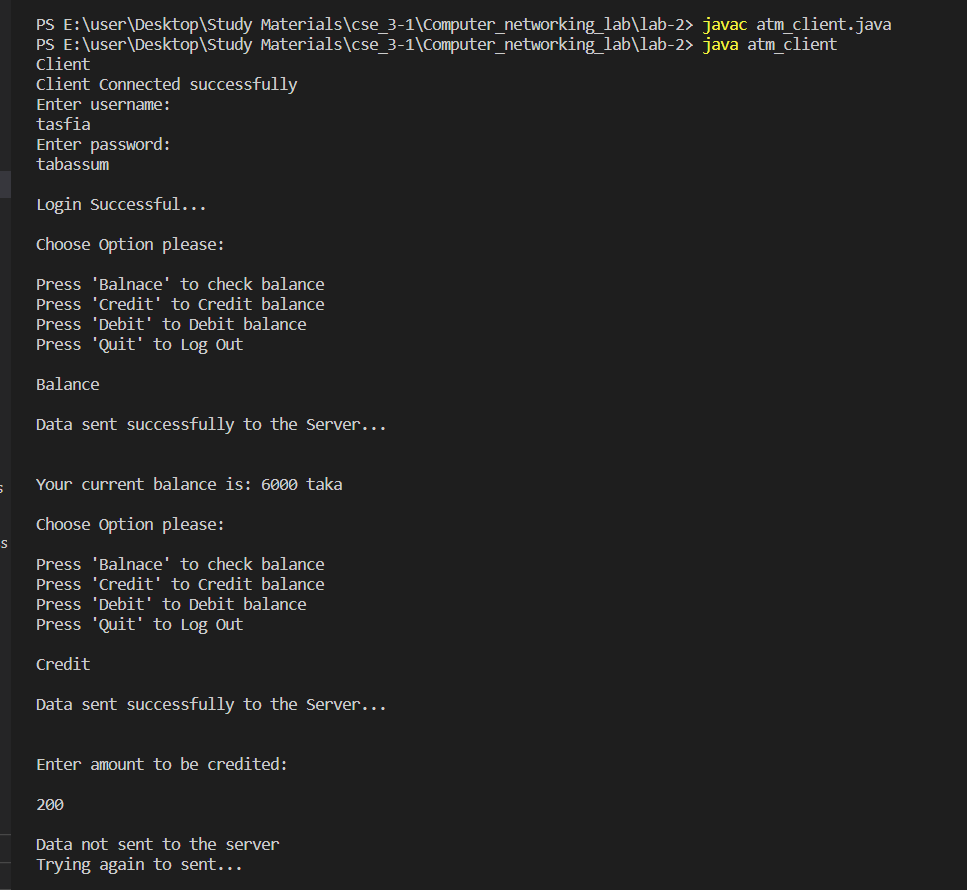
\includegraphics[width=\textwidth]{atm_client1.png}
\caption{ATM Client}
\end{figure}
\begin{figure}[!h]
\centering
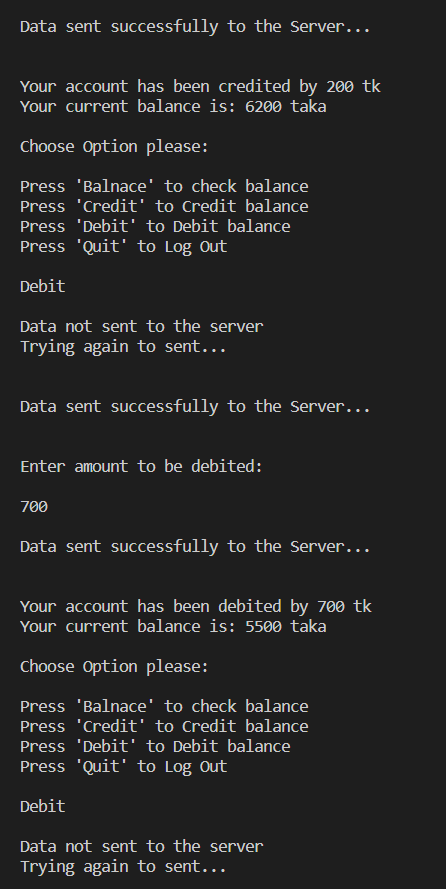
\includegraphics[width=\textwidth,height=14cm,keepaspectratio]{atm_client2.png}
\caption{ATM Client}
\end{figure}
\begin{figure}[!h]
\centering
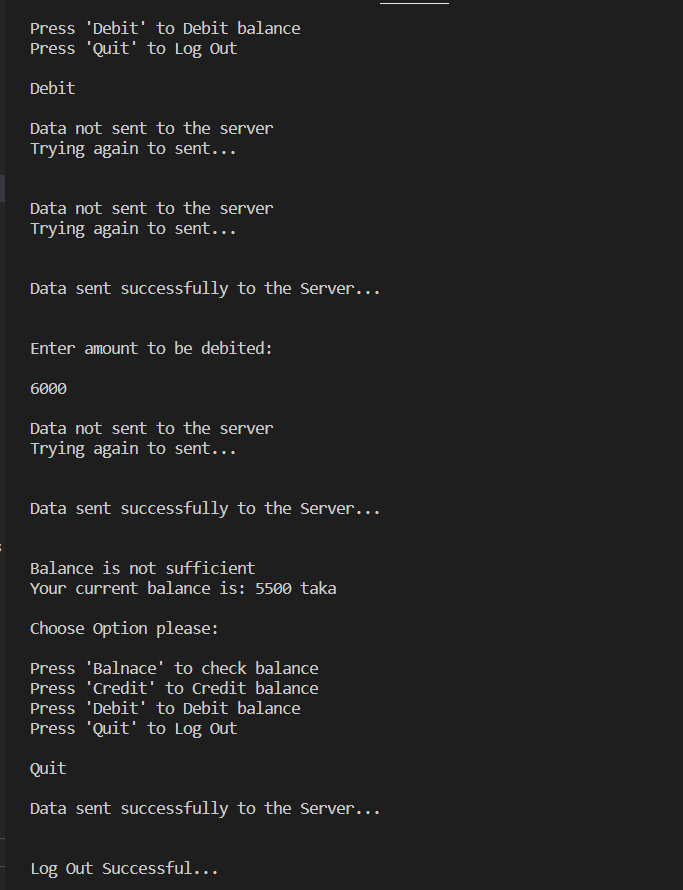
\includegraphics[width=\textwidth,height=14cm,keepaspectratio]{atm_client3.png}
\caption{ATM Client}
\end{figure}
\FloatBarrier


\textbf{There are mail four parts :} \\[12pt]
- User first Connect with server\\[2pt]
-User Can login Using Username and Password\\[2pt]
-Then A User Can Check Balance,Credit, Debit, And if user Want can logout.
-In the error part if the data cann't be sent in a time and will give an error and will resend the data.
\section{Source Code :}
\url{https://github.com/Saimatonni/Computer_Networking}



\section{Experience}
\begin{enumerate}
   \item Here we have learned about socket programming.
    \item We had also gone through various examples of client-server communication. For this, we have used Visual Studio Code for IDE.
    \item We have come to know about how through client-server communication we can send information from client to server and then receive the expected result from it.
\end{enumerate}
\begin{thebibliography}{1}
\bibitem{book}  Computer networking : a top-down approach 6th ed.
\bibitem{StackOverflow} StackOverflow : \url{https://stackoverflow.com/questions/64718872/tcp-server-and-client-in-java}
\bibitem{geeksforgeeks} GeeksforGeeks : \url{https://www.geeksforgeeks.org/socket-programming-in-java/}
\bibitem{tutorial} YouTube Tutorial :\url{https://www.youtube.com/watch?v=vCDrGJWqR8w/}
\end{thebibliography}
\end{document}
